% Caution!!! Only compilable with XeLaTx, one will encounter strange error when using pdflatex.

% Compile environment: miktex portable ver.2.9; Partly tested on Linux texlive

% jarticle is not available for xelatex... Which means the spacing and line changing should be done in mannual way...
\documentclass[a4,12pt]{article}

% use xeCJK otherwise line changing cannot be done.
\usepackage{xeCJK}

% If you want to try otf font...
\usepackage{xltxtra}

% In order to modifying the line spacing. In text insert \setstretch{1.0}
\usepackage{setspace}

% Heart of xelatex. In order to utilize ttf and ttc font.
\usepackage{fontspec}

% In order to display the symbol: celsius degree.
\usepackage{gensymb}

% To insert graphics inside text.
\usepackage{graphicx}

% To modify the page style (space). Spacing style is compared with YoshidaS 3rd year paper.
\usepackage[top=1in, bottom=1.5in, left=1.4in, right=1.4in]{geometry}

% A mincho Japanese font developed by IPA. IPAex includes a Gothic and a Mincho font.
%\setCJKmainfont[ Path = fonts/]{ipaexm.ttf}
% For english characters and numbers, Times New Roma seems to be perfect.
%\setmainfont[ Path = fonts/]{times.ttf}

% By default latex do NOT indent the first paragraph.
% To indent a paragraph besides the first one, add \par to the leading paragraph.
\usepackage{indentfirst}

% Set path for saving all the figures and graphs
% Don't forget to update this address if you move the whole working directory
% 1. Do not include white space within.
% 2. Do not forget to include a "/" at the end of the addr.
\graphicspath{{./Figures/}}

% For using bibtex and biber
% 1. sorting=none to override default sorting.
% 2. style= *, to choose a biblo style
%\usepackage[
%sorting=none,
%style=numeric,
%isbn=false,
%doi=false,
%]{biblatex}
%\addbibresource{references.bib}

% In order to customize the Figure and Table caption style.
% 1. Use white space instead of colon.
% 2. Add period at the end of each caption.
% ftp://ctan.tug.org/tex-archive/macros/latex/contrib/caption/caption-eng.pdf
\usepackage[
tableposition=top,
labelsep=space,
textformat=period,
]{caption}

% In order to write some calculation equations without numbering them 
\usepackage{mathtools}

% In order to creat /  generate a list of symbols
\usepackage{nomencl}
\makenomenclature

% In order to print the symbol of Laplace transformation curly L
\usepackage{ amssymb }

% To display url correctly in Bibtex (?) May not be necessary...
\usepackage{url}

% To embed Python script in LaTex...
\usepackage{python}

\begin{document}

\include{title}
% Compared with YoshidaS 3rd year paper. 1.2 seems to be fine...
\setstretch{1.2}

\title{geekhead}
\author{houkensjtu}
\date{2016.6.30}
\maketitle
\section {New}
A backbone directory structure.
\begin{figure}[h]
\begin{center}
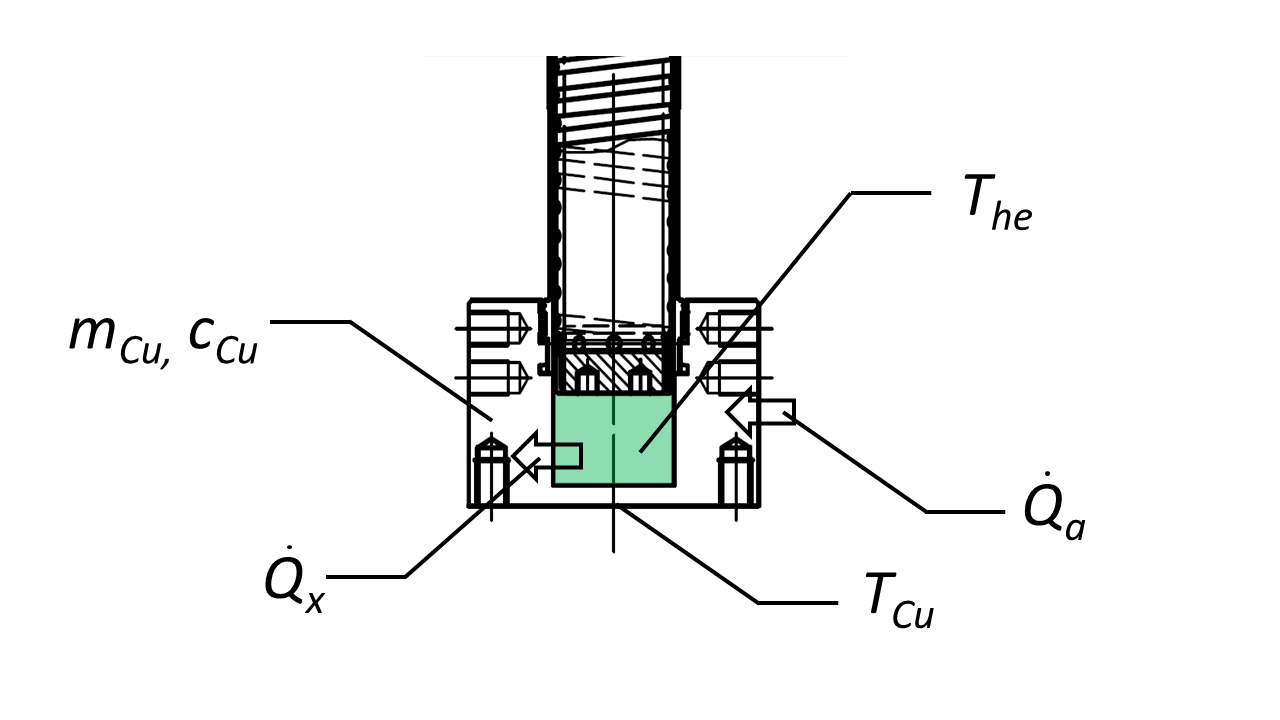
\includegraphics[width=13cm]{coldhead_behavior.png}
\caption{A schematic drawing of cold head.}
\end{center}
\end{figure}


%Notes on how to compile references in bibtex:
%1. Compile main.tex by xelatex, this generate a bunch of .aux files
%2. Compile main.tex by biber, this generate main.bll and main.blg file
%3. Compile main.tex again by xelatex, now the reference should display at the end
%4. Compile main.tex with xelatex one more time...

%Extra note:
%Bibtex will sort the references in different order so use unsrt to override
%authors should all be connected with the word and, not comma

%\bibliographystyle{unsrt}
%\bibliography{sample}
\printnomenclature

\end{document}
